% \documentclass[14pt]{extarticle}
\documentclass[12pt]{article}
\usepackage[margin=0.1in]{geometry}
\usepackage{xcolor}
\usepackage{framed}
\usepackage{enumitem}
\usepackage{mathtools,xparse}
\colorlet{shadecolor}{orange!15}
% \definecolor{shadecolor}{rgb}{255,128,0}\
\usepackage{float}
\usepackage{fullpage} % Package to use full page
\usepackage{parskip} % Package to tweak paragraph skipping
\usepackage{tikz} % Package for drawing
\usepackage{amsmath}
\usepackage{amssymb}
\usepackage{hyperref}
\usepackage{graphicx} % Allows including images
\usepackage{booktabs} % Allows the use of \toprule, \midrule and \bottomrule in tables
\usepackage{longtable} %Allows multi-column tables 

\allowdisplaybreaks
\setlength{\parindent}{3em}
\setlength{\parskip}{1em}
\renewcommand{\baselinestretch}{1.5}

\newcommand{\toP}{\overset{p}{\to}}
\newcommand{\meanN}{\frac{1}{n}\sum_{i=1}^n}
\newcommand{\sumL}{\sum_{\ell=1}^{L_i}}
\newcommand{\meanL}{\frac{1}{L_i}\sumL}
\newcommand{\sumJ}{\sum_{j=1}^{J_i}}
\DeclarePairedDelimiter{\norm}{\lVert}{\rVert}
\usepackage{setspace}
% \doublespacing
\usepackage[english]{babel}
\usepackage[utf8x]{inputenc}
% \title{$M_{4,k}$}
% \author{}
\date{\vspace{-30pt}\today}

\begin{document}
\begin{center}
\Large{\singlespacing Notes on Imperfect Matching Paper \\ 
Rachel Anderson \\
\today \\}
\end{center} 
% \maketitle
\section{Setup}
The goal is to estimate $\theta_0$ that satisfies the model
\begin{equation} E_0[m(y_i, x_i, z_i; \theta_0)]  \label{model} \end{equation}
where the expectation is taken with respect to the joint distribution $f_0(y, x,z)$.  Instead of observing a random sample $(y_i,x_i,z_i)$ drawn from $f_0(y,x,z)$, the econometrician observes two random samples drawn from $f_0(y)$ and $f_0(x,z)$ independently.  

The first sample contains $(x_i, z_i, w_i)_{i=1}^n$, where $(x_i, z_i)$ are drawn from the marignal distribution $f_0(x,z)$.   The second contains outcomes $(\{y_{i\ell}\}_{\ell = 1}^{L_i}, w_i)_{i=1}^n$, that are linked to $(x_i, z_i)$ by the identifier $w_i$, which also appears in the first dataset.  The econometrician believes that only one of the $\{y_{i\ell}\}_{\ell=1}^{L_i}$ is drawn from the distribution $f(y_i^* | x_i^*, z_i^*)$; the other outcomes are spurious matches that arise because the identifying information $w_i$ is insufficent to form unique data tuples. 

To fix ideas, suppose the econometrician would like to estimate the impact of a single mother assistance program on participants' children's longevity (call this unknown parameter $\theta$).  The researcher collects two datasets; the first consists of aid program applications, with variables about mother and child characteristics $(x_i^*, z_i^*)$ and the child's first and last names, and place and year of birth $(w_i)$.  The second data set contains death records (used to construct $y_i^*$), and is indexed by the individual's first and last names, and place and year of birth $(w_i)$.    

Although individuals with distinct names are unlikely to appear on multiple death records, individuals with common names like ``John Smith" may be linked to multiple death records.  Similarly, if the econometrician matches individuals using a subset of the variables in $w_i$ (as in the case that females are matched by first name only, and place and year of birth), she is likely to find many possible links that are equally credible.  

The following note formalizes the assumptions that are necessary to estimate the model ($\ref{model}$) without dropping observations with non-unique matches.


\textbf{Assumption 1.} The observed $(x_i, z_i, w_i)$ is a random sample drawn from the marginal distribution $f(x^*, z^*, w^*)$.   The $\{y_{i\ell}\}_{\ell=1}^{L_i}$ is a random sample drawn from $f(y^* | w_i, L_i)$, so that $(x_i, z_i) = (x_i^*,z_i^*)$ and $y_{i\ell}$ are independent conditional on $w_i$ for $y_{i\ell} \neq y_i^*$. 

\textbf{Assumption 2.}  There is exactly one $y_{i\ell} = y_i^*$, $\ell\in \{1, \dots, L_i\}$ for all $i.$ That is, we assume that one of the $\{y_{i\ell}\}_{\ell=1}^{L_i}$ is drawn from the marginal distribution $f(y_i^* | x_i^*, z_i^*) = f(y_i^* | x_i, z_i)$.   

This assumption implies we can write $y_i^* = \sum_{\ell=1}^{L_i} s_{i\ell} y_{i\ell}$, where $s_{i\ell}$ is an unobserved latent variable that equals 1 if $(y_{i\ell}, x_i, z_i) = (y_i^*, x_i^*, z_i^*)$, and that equals 0 otherwise.  
Also, $\sum_{\ell=1}^{L_i} s_{i\ell} = 1$ for all $i$, and we can rewrite \ref{model} as,
\begin{equation} E\left[m(y_i^*, x_i^*, z_i^*)\right] = 0 \iff E\left[m(y_{i\ell},x_i,z_i; \theta_0) | s_{i\ell} =1 \right] = 0  \tag{$1^*$} \label{truemodel} \end{equation} 

\textbf{Assumption 3}. The identifying variables $w_i$ in $(x_i, z_i, w_i)$ exactly match, or are sufficiently close to $w_i$ in $(\{y_{i\ell}\}_{\ell=1}^{L_i}, w_i)$, such that the researcher cannot distinguish which $y_{i\ell} = y_i^*$ for $\ell \in \{1, \dots, L_i\}$.  In other words, the researcher behaves as if,  
$$P(s_{i\ell}=1 | w_i, L_i) = \frac{1}{L_i}$$ 
Assumptions 1 and 3 rule out unobserved sample selection, in the sense that all individuals with the same identifying information have equal probability of appearing in the sample.  This assumption would be violated if, for example, higher income individuals have a greater probability of appearing in the sample, unless $w_i$ includes income.   

\section{Estimating $\theta$}

The goal is to estimate (\ref{truemodel}) without observing the $s_{i\ell}$. One thing we can do is evaluate the moment conditions $m(\cdot)$ for each  $y_{i\ell}$ in the sample.  Hence, we consider (ignoring $z_i$ for simplicity):
\begin{align*}
    E\left[\sumL m\left(y_{i\ell}, x_i; \theta\right) \Bigg\vert w_i, L_i, \right] &=
    \sumL \Big\{ E[m(y_{i\ell}, x_i; \theta) | w_i, L_i, s_{i\ell}=1]P(s_{i\ell}=1| w_i, L_i) 
    \\&+ E[m(y_{i\ell}, x_i; \theta) | w_i, L_i, s_{i\ell}=0] P(s_{i\ell}=0| w_i, L_i) \Big\}
\end{align*}
   
By Assumption 1, $P(s_{i\ell} = 1 | w_i, L_i) = \frac{1}{L_i}$, so that 

\begin{align*}  E\left[\sumL m\left(y_{i\ell}, x_i; \theta\right) \Bigg\vert w_i, L_i, \right]  &= \meanL E[m(y_{i\ell}, x_i; \theta) | w_i, L_i, s_{i\ell} = 1] \\&+ \frac{L_i-1}{L_i}E[m(y_{i\ell}, x_i; \theta) | w_i, L_i, s_{i\ell} = 0] \end{align*}
and random sampling implies the expectations are equal for all $i$, 
\begin{equation*}
   E\left[\sumL m\left(y_{i\ell}, x_i; \theta\right) \Bigg\vert w_i, L_i, \right] = E\left[m(y_{i\ell}, x_{i}; \theta) | w_i, L_i, s_{i\ell} = 1\right] + (L_i - 1)E\left[m(y_{i\ell}, x_i; \theta) | w_i, L_i, s_{i\ell} =0 \right] 
\end{equation*}
Rearranging terms, 
\begin{equation*} E[m(y_{i\ell}, x_i; \theta) | w_i, L_i, s_{i\ell}=1] = E\left[\sum_{\ell=1}^{L_i} m(y_{i\ell},x_i; \theta)\Bigg\vert w_i, L_i \right] - (L_i-1) E[m(y_{i\ell},x_i; \theta) | w_i, L_i, s_{i\ell} = 0] \end{equation*}
Note that $E[m(y_{i\ell}, x_i; \theta) | w_i, L_i, s_{i\ell} = 0]$ is an expectation with respect to the distribution of false matches.  In this case, $y_{i\ell} \neq y_i^*$ is independent of $x_i^* = x_i$ conditional on $w_i$, so that
$$ E[m(y_{i\ell}, x_i; \theta) | w_i, L_i, s_{i\ell} = 0] =  E[m(y_{i\ell}, x_i; \theta) | w_i, L_i, x_i, s_{i\ell} = 0] \equiv g(w_i, L_i, x_i; \theta)$$ 
Finally, by the Law of Iterated Expectations,
\begin{equation}
E[m(y_{i\ell}, x_i; \theta) | s_{i\ell}=1] = E\left[\sum_{\ell=1}^{L_i} m(y_{i\ell},x_i; \theta)\right] -  E[(L_i -1)g(w_i,L_i,x_i, \theta)]
\end{equation}
which we can approximate with the sample analog:
\begin{equation} \hat{E}\left[m(y_{i\ell}, x_i; \theta) | s_{i\ell} =1\right] = \meanN \sumL m(y_{i\ell}, x_i; \theta) -  \meanN(L_i - 1) \hat{g}(w_i, L_i, x_i; \theta) \label{moments} \end{equation} 
where $n$ is the number of observations in the $(x_i, z_i, w_i)$ file, and $\hat{g}$ is a parametric or nonparametric estimate of $g(\cdot).$  
Estimation proceeds as usual by applying GMM to \ref{moments} as the sample moments.    


\section{Large Sample Results}
Define the estimator 
\begin{gather} \hat{\theta} =  \underset{\theta \in \Theta}{\arg\min}\ m_n(\theta, \hat{g})'\hat{W}m_n(\theta,\hat{g}) \\
m_n(\theta,\hat{g}) = \meanN \sum_{\ell=1}^{L_i} m(y_{i\ell}, x_i, z_i; \theta) - (L_i -1) \hat{g}(x_i, z_i, w_i, L_i; \theta) 
\end{gather}

where $\hat{g}(\cdot)$ is a nonparametric estimator of $g(\cdot)$.   Let also $ m(\theta) \equiv m(y_i,x_i,z_i;\theta)$.


\textbf{Theorem 1 (Consistency)}.  If the following assumptions are true,
\begin{enumerate} \item  $\left(x_i,z_i,w_i, \{y_{i\ell}\}_{\ell=1}^{L_i}\right)_{i=1}^n$ is a random sample, and $\{y_{i\ell}\}_{\ell = 1}^{L_i}$ and $(x_i, z_i)$ are i.i.d. samples conditional on $w_i$
\item $\hat{W} - W = o_p(1)$, $W$ is positive semi-definite, $WE[m(y_i,x_i, z_i; \theta)] = 0 $ has a unique solution on $\Theta$ at $\theta_0$, with $\Theta$ a compact subset of $\mathcal{R}^d$.
\item (i) $m(y_{i\ell}, x_i, z_i, \theta)$ is continuous at each $\theta \in \Theta$ with probability 1; \\(ii) $E\left[\sup_{\theta\in\Theta} || \sum_{\ell=1}^{L_i} m(y_{i\ell}, x_i, z_i, \theta) || \right] < \infty$; \\
(iii) $\sup_{\theta}\lVert \hat{g}(x_i,z_i,w_i,L_i;\theta)- g(x_i,z_i,w_i, L_i;\theta) \rVert \toP 0 $. 
\end{enumerate} 
then $\hat{\theta} \toP \theta_0$. 

\textbf{Proof.} Assumption 2 is the ID condition for GMM.  To apply Theorem 2.1 in Newey \& McFadden (1994), we verify uniform convergence of the sample objective function.

Define $\hat{Q}_n(\theta) = m_n(\theta,\hat{g})' \hat{W} m_n(\theta,\hat{g})$, and $Q_0(\theta) = E[m(\theta)]'WE[m(\theta)]$. Assumptions 1-3 and (7) imply
\begin{align*}
    \sup_{\theta} \left\lVert m_n(\theta,\hat{g}) - E[m(\theta)] \right\rVert &\leq \sup_{\theta} \left\lVert \meanN \sum_{\ell=1}^{L_i} m(y_{i\ell}, x_i, z_i, \theta) - E\left[\sum_{\ell=1}^{L_i}m(y_{i\ell},x_i,z_i; \theta)\right] \right\rVert  \\
    &+ \sup_{\theta} \left\lVert \meanN (L_i-1) \hat{g}(x_i,z_i,w_i,L_i; \theta) - E\left[(L_i - 1) g(x_i, z_i, w_i, L_i; \theta)\right] \right\rVert \\
    &\leq o_p(1) + \sup_{\theta} \left\lVert \meanN (L_i -1)\left(\hat{g}(x_i, z_i, w_i, L_i; \theta) - g(x_i, z_i, w_i, L_i; \theta)\right) \right\rVert \\&+ \sup_{\theta} \left\lVert \meanN (L_i-1) g(x_i, z_i, w_i, L_i;\theta) - E[(L_i - 1) g(x_i, z_i, w_i, L_i;\theta)\right\rVert \\
    &\leq \meanN (L_i -1) \sup_{\theta} \left\lVert \left(\hat{g}(x_i, z_i, w_i, L_i; \theta) - g(x_i, z_i, w_i, L_i; \theta)\right) \right\rVert + o_p(1)= o_p(1)
\end{align*}
The remainder of the proof showing $\sup_{\theta} \lVert\hat{Q}_n(\theta) - Q(\theta)\rVert$ follows from the generic proof for GMM consistency. $\square$


Note that the second part of Assumption 1 is necessary to derive the estimator.  Assumption 2 is the standard identification assumption for GMM, and Assumption 3 assures uniform convergence of the  objective function.  If $\hat{g}$ is a sieve estimator, the conditions in Chen, Hong, and Tamer (2005) can be used to replace Assumption 3(iii). 



\textbf{Theorem 2 (Asymptotic Normality)} If, in addition to Assumptions 1-3, the following are true,
\begin{enumerate}[resume]
    \item $\theta_0 \in \text{int}(\Theta)$
    \item $G(\theta) \equiv E\left[\nabla_{\theta} m(\theta)\right] = E\left[\frac{\partial}{\partial \theta'} \left\{ \sum_{\ell=1}^{L_i} m(y_{i\ell}, x_i,z_i; \theta) - (L_i -1)g(\cdot\ ;\theta)\right\}\right]$ is continuous at $\theta_0$ and $\sup_{\theta\in \mathcal{N}} \left\lVert \nabla_{\theta}m_n(\theta,\hat{g}) - G(\theta)\right\rVert \toP 0 $ where $\mathcal{N}$ is a neighborhood of $\theta_0$
    \item For $G=G(\theta_0)$, $G'WG$ is nonsingular 
    \item $E\left[m(y_i, x_i, z_i; \theta)m(y_i, x_i, z_i; \theta)\right]$ is finite, positive definite, which is also written as
$$\hspace{-30pt} E\left[\left\{\sum_{\ell=1}^{L_i} m(y_{i\ell},x_i, z_i; \theta) - (L_i -1) g(x_i,z_i, w_i, L_i; \theta)\right\} \left\{ \sum_{\ell=1}^{L_i} m(y_{i\ell},x_i, z_i; \theta) - (L_i -1) g(x_i,z_i, w_i, L_i; \theta)\right\}'\right] $$
\item $\hat{g}(\cdot)$ satisfies regularity conditions (specifically, stochastic equicontinuity and mean-square continuity) so that $n^{1/2}m_n(\theta_0, \hat{g}) \Rightarrow \mathcal{N}(0,\Omega)$, with

$$ \Omega = \text{Avar}\left(\frac{1}{\sqrt{n}}\sum_{i=1}^n \left( \sum_{\ell =1}^{L_i} m(y_{i\ell}, x_i, z_i; \theta_0) - (L_i-1) \hat{g}(x_i, z_i, w_i; \theta_0)\right)  \right) $$

\end{enumerate}

then $\sqrt{n}(\hat{\theta}-\theta_0) \Rightarrow \mathcal{N}(0,V)$, where 
\begin{equation} V = (G'WG)^{-1}G'W\Omega W G(G'WG)^{-1} \label{avar}\end{equation}

\textbf{Proof.} Mean-value expansion and first-order conditions imply:
\begin{align*} \sqrt{n}(\hat{\theta}-\theta_0) &= (\nabla_{\theta}m_n(\bar{\theta},\hat{g})' \hat{W} \nabla_{\theta} m_n(\hat{\theta},\hat{g}))^{-1}  \nabla_{\theta} m_n(\hat{\theta},\hat{g})' \hat{W} \frac{1}{\sqrt{n}}\sum_{i=1}^n m_n(\theta_0,\hat{g})\\
&= (G'WG)^{-1}G'W\frac{1}{\sqrt{n}}\sum_{i=1}^n m_n(\theta_0,\hat{g}) + o_p(1)
\end{align*}
where \begin{align*}
     \frac{1}{\sqrt{n}} \sum_{i=1}^n m_n(\theta_0,\hat{g}) &= \underbrace{\frac{1}{\sqrt{n}} \sum_{i=1}^n \left( \sum_{\ell =1}^{L_i} m(y_{i\ell}, x_i, z_i; \theta_0) - (L_i - 1) g(x_i,z_i, w_i, L_i; \theta_0)\right)}_{\Rightarrow \mathcal{N}(0, E[m(\theta_0)m(\theta_0)'])}  \\&+ \frac{1}{\sqrt{n}}\sum_{i=1}^n (L_i-1)\left(g(x_i,z_i,w_i,L_i; \theta_0) - \hat{g}(x_i,z_i,w_i,L_i;\theta_0)\right)  
 \end{align*}
To show that $\frac{1}{\sqrt{n}}\sum_{i=1}^n m_n(\theta_0,\hat{g}) \Rightarrow \mathcal{N}(0, \Omega)$, we verify the conditions in Theorem 8.1 in Newey \& McFadden (1994):

\begin{enumerate}
    \item Linearization is immediate\footnote{with $G(z,g-g_0) = z_i(L_i-1)(g_0-\hat{g})$} because $m_n$ is linear in $g(\cdot)$
    \item Stochastic equicontinuity requires, for the true distribution of the data $F_0$ , 
    $$\frac{1}{\sqrt{n}}\left[\sum_{i=1}^n  (L_i-1)(g-\hat{g}) - \int (L_i-1)(g-\hat{g}) d F_0 \right] \toP 0 $$ 
    \item (Mean-square differentiability) (i) there is $\delta(z)$ and a measure $\hat{F}$ s.t. $E[\delta(z)] = 0, \ E[\lVert \delta(z)\rVert^2] < \infty $, and for all $\lVert g-\hat{g}\rVert$ small enough, $\int (L_i-1)(g-\hat{g})dF_0 = \int \delta(z) d \hat{F}$
    \item For the empirical distribution $\tilde{F}, \sqrt{n}\left[\int \delta(z)d\hat{F} - \int \delta(z) d\tilde{F}\right] \toP 0$
\end{enumerate}

Then $\frac{1}{\sqrt{n}}\sum_{i=1}^n m_n(\theta_0,\hat{g}) \Rightarrow \mathcal{N}(0, \Omega)$, where $\Omega = \text{Var}[m(\theta_0) + \delta(z)].\ \square$

 

Assumptions 4-7 are the usual regularity and dominance conditions to ensure $\sqrt{n}$-normality of the GMM estimator of $\theta_0$ when $g(\cdot)$ is known.  Using instead a non-parametric estimator $\hat{g}$, such as a sieve estimator, requires additional regularity conditions, such as those outlined in the proof and in Chen, Hong and Tamer (2005). 
\subsection*{Example: Linear Instrumental Variables} 
The model is \begin{equation} m(y_i, x_i, z_i; \theta) = z_i(y_i-x_i'\beta) \end{equation}

The $g(\cdot)$ nonparametric function becomes, 
$$ g(x_i, z_i, w_i, L_i;\theta) = z_i\left(E[y_{i\ell} | w_i, L_i] - x_i'\beta\right)$$
An estimate of $\hat{g}(\cdot)$ replaces $E[y_{i\ell} | w_i, L_i]$ with $\hat{E}[y_{i\ell} | w_i, L_i]$.  

% So we have 
% \begin{align*}
%     E[z_i(y_i-x_i'\beta)] &= E\left[ \sum_{\ell=1}^{L_i} z_i (y_{i\ell} - x_i'\beta) \right] - E\left[(L_i - 1) g(x_i,z_i, w_i,L_i;\theta)\right] \\
%     &= E\left[ z_i \left(\sum_{\ell=1}^{L_i} y_
%     {i\ell} - (L_i-1) E[y_{i\ell} | w_i, L_i] - x_i'\beta\right)\right] \\
%     &= E\left[z_i\left(E[y_{i\ell} | w_i, L_i] + \sum_{\ell=1}^{L_i}(y_{i\ell} - E[y_{i\ell} | w_i, L_i])\right)  - z_ix_i'\beta\right]
% \end{align*}

% *Is there a connection with FE? 


When the model is over-identified, i.e. dim$(z_i) > $ dim$(x_i)$, the estimator is 
\begin{gather*}
    \hat{\beta} = \left( \meanN P z_ix_i' \right)^{-1} \meanN Pz_i\left(\sum_{\ell = 1}^{L_i} y_{i\ell} - (L_i - 1) \hat{g}(w_i,L_i,\beta) \right)
\end{gather*}
where $P$ is a weighting matrix, and choosing $P$ is equivalent to choosing $W$ in GMM. 
For identification, we replace Assumption 2 with 

\textbf{Assumption 2'.}  $PE[z_ix_i']$ exists and is nonsingular,

 Additionally, we do not need Assumption 3(i) since $m(\cdot)$ is linear in $\beta$.  Assumption 3(ii) will be satisfied if  $E[z_i\sum_{\ell=1}^{L_i}y_{i\ell}]<\infty$.  

\textbf{Corollary (Consistency).}  If (i) $(x_i,z_i, w_i, \{y_{i\ell}\}_{\ell=1}^{L_i})_{i=1}^n$ is a random sample, and $\{y_{i\ell}\}_{\ell=1}^{L_i}$ and $(x_i,z_i)$ are random samples conditional on $w_i$, (ii) $PE[z_ix_i']$ exists and is nonsingular, (iii) $E[z_i\sum_{\ell=1}^{L_i}y_{i\ell}]<\infty$, and (iv) $\sup_{\theta} \left\lVert \hat{g}(w_i, L_i) - g(w_i, L_i) \right\rVert \toP 0$, then $\hat{\beta}\toP \beta_0$. 

The statement is proved by verifying the assumptions of Theorem 1. 

\textbf{Corollary (Asymptotic Normality)} If in addition to (i)-(iv) above, $\hat{g}(\cdot)$ satisfies regularity stochastic equicontinuity and mean-square differentiability, then $\sqrt{n}(\hat{\beta}-\beta_0) \Rightarrow \mathcal{N}(0, V)$, where $V$ is defined as in (\ref{avar}) with $G= PE[z_ix_i']$ and 
$$\Omega = \text{Avar}\left( \frac{1}{\sqrt{n}}\sum_{i=1}^n z_i \left(\sum_{\ell=1}^{L_i} y_{i\ell} - (L_i-1)\hat{g}(w_i,L_i,\beta)\right)\right) $$ 

As before, the asympotic variance formula depends on the choice of $\hat{g}(\cdot)$.  In a later section, we derive exact formulas for a kernel estimator of $\hat{g}$.  

\section{Estimating Asymptotic Variance}

As usual, a consistent estimator of (\ref{avar}) can be formed by plugging in estimators of the different pieces.  An estimator of $G$ can be formed in a straightforward way:
$$ \hat{G} = \meanN \nabla_{\theta} m_n(\hat{\theta}) = \meanN \left(\sum_{\ell=1}^{L_i}\nabla_{\theta} m(y_{i\ell}, x_i, z_i; \hat{\theta}) - (L_i-1) \nabla_{\theta}\hat{g}(x_i, z_i, w_i, L_i; \hat{\theta})\right)$$ 
which is consistent under the same conditions used for asymptotic normality of $\hat{\theta}$. 

The more difficult term to estimate is the ``score" variance $\Omega$.  One estimator, suggested in Newey \& McFadden (1994), uses an estimator $\hat{\delta}(z)$ of the function $\delta(z)$,

$$\hat{\Omega} = \meanN \left\{m(y_{i},x_i,z_i; \hat{\theta}) + \hat{\delta}(z_i)\right\}\left\{m(y_{i},x_i,z_i; \hat{\theta}) + \hat{\delta}(z_i)\right\}'$$

If, in addition to the assumptions of Theorem 1,  $\meanN \left\lVert m_n(\hat{\theta}, \hat{g}) - m( \theta_0) \right\rVert^2 \toP 0$, and $\meanN \left\lVert \hat{\delta}(z_i)-\delta(z_i)\right\rVert^2\toP 0$ then $\hat{\Omega} \toP \Omega$ by Lemma 8.3 in Newey \& McFadden (1994).  

Hence, by Slutsky's and the continuous mapping theorem,
$$ \hat{V} = (\hat{G}'\hat{W}\hat{G})^{-1} \hat{G}'\hat{W}\hat{\Omega} \hat{W}\hat{G} (\hat{G}'\hat{W}\hat{G})^{-1} \toP (G'WG)^{-1}G'W\Omega W G (G'WG)^{-1} = V$$  


% \section{Exact formulas for Linear IV with Kernel} 

% A nonparametric kernel estimator of $g$ is $$\hat{g}(w) = \frac{\sum_{i=1}^n \sumL y_{i\ell} K_{\sigma}(w-w_{i\ell})}{\sum_{i=1}^n \sumL K(w-w_{i\ell})}$$
% where $K_{\sigma}(v) = \sigma^{-r} K(v/\sigma)$, $r$ is the dimension of $w$, $K(u)$ is a function such that $\int K(u) du =1$, and $\sigma$ is a bandwith term chosen by the econometrician.  Following Newey \& McFadden we write $\hat{g}(w) = \frac{\hat{\gamma}_2(w)}{\hat{\gamma}_1(w)}$.  

% The estimator is of the form $\meanN g(z_i, \theta, \hat{\gamma}) = 0$ where $g(z_i, \theta, \gamma) = z_i \left(\sumL y_{i\ell} - x_i'\beta - (L_i-1)\gamma(w)\right)$.  Let also $g(z_i, \gamma) = g(z_i, \theta_0, \gamma)$.  

% The linearization condition in Theorem 8.1 is satisfied by choosing $ G(z, \gamma - \gamma_0) = z_i(L_i-1)(\gamma-\gamma_0)$, so that

% $$\left\lVert g(z, \gamma) - g(z, \gamma_0) - G(z, \gamma-\gamma_0) \right\rVert = 0 \leq \lVert \gamma(w) - \gamma_0(w) \rVert^2 $$

% Hence assumption (i) of Theorem 8.1 will be satisfied if $\sqrt{n}\sup_{w} \lVert \hat{\gamma}(w) - \gamma_0(w)\rVert^2 \toP 0 $.  When $\hat{\gamma}$ is a kernel estimator defined above, we require that $\gamma_{10} = f_0(w)$ is bounded away from zero, $\gamma_{20}(w)$ is bounded, and $\gamma_1(w)$ is uniformly close to $\gamma_{10}(w)$  (Alternatively, because the remainder term equals zero, this does not matter at all? Newey gives many regularity conditions, such as $K(u)$ is differentiable of order $d$, the derivatives of order $d$ are bounded, $K(u)$ is zero outside a bounded set, etc.)

% Assumption 2 in Theorem 8.1 (Stochastic equicontinuity) results from $G(z,\gamma)$ linaer in $\gamma$ and a small bias condition. Assumption 3 (mean square differentiability) follows by setting $v(x) = 1$




\section{Bootstrap}

The estimator proposed in this paper is a two-step semiparametric GMM estimator, where the first step involves estimating the control function $g$.  As shown by Theorem 2, the resulting estimator is asymptotically linear and asymptotically normal, so it satisfies the regularity conditions in Mammen (1992) that guarantee validity of the nonparametric bootstrap.  More specifically, the nonparametric bootstrap is consistent under the regularity conditions for a (potentially over-identified) standard GMM model specified in Hahn (1996, Theorem 1), when $g$ is known. 
 

The bootstrap is especially useful When $\hat{g}$ is estimated, as deriving $\Omega$ in the asymptotic variance formula may be difficult.  In this case, the researcher should shrink the kernel bandwidth to reduce asymptotic bias (Horowitz, 2001).  

Depending on the model, other bootstrap methods may be valid.  For example, residual bootstrap (I think) would work for linear IV. 

\section{Bias-variance tradeoff}

Suppose we are trying to estimate the mean of a random variable $X \sim \mathcal{N}(\mu, \sigma^2)$, however for each member of the sample $i$ we collect two observations, $X_{i1}, X_{i2}$.  Suppose we know that the first observation is drawn from the true distribution of $X$ with probability $\pi$; with probability $1-\pi$, $X_{i1} \sim \mathcal{N}(\kappa, \omega^2)$.  The two observations are dependent, so that when $X_{i1}$ is drawn from the incorrect distribution, $X_{i2}$ is drawn from the correct distribution, and vice versa.
e
For $(\mu, \sigma^2)=(0,1)$ and $(\kappa, \omega^2) = (0,4)$ I solve for $(a_2, a_3)$ that give an  unbiased estimator of $\hat{\mu}$ using the formulas in the paper.  For $n=100$, $\pi \in (0.1, 0.9)$, and $a_1 \in \{1, \dots, 10\}$, I plot the bias and variance of $\hat{\mu}$ that result from having beliefs $\hat{\pi}\neq \pi$.  

When $a_1 = a_2 = a_3 = 1$, the bias is 0. Figure 1 shows my results for $a_1 = 2$.

\begin{figure}[h!]
    \centering
    \caption{Bias-Variance Tradeoff varying $\hat{\pi}$ and true $\pi$}
    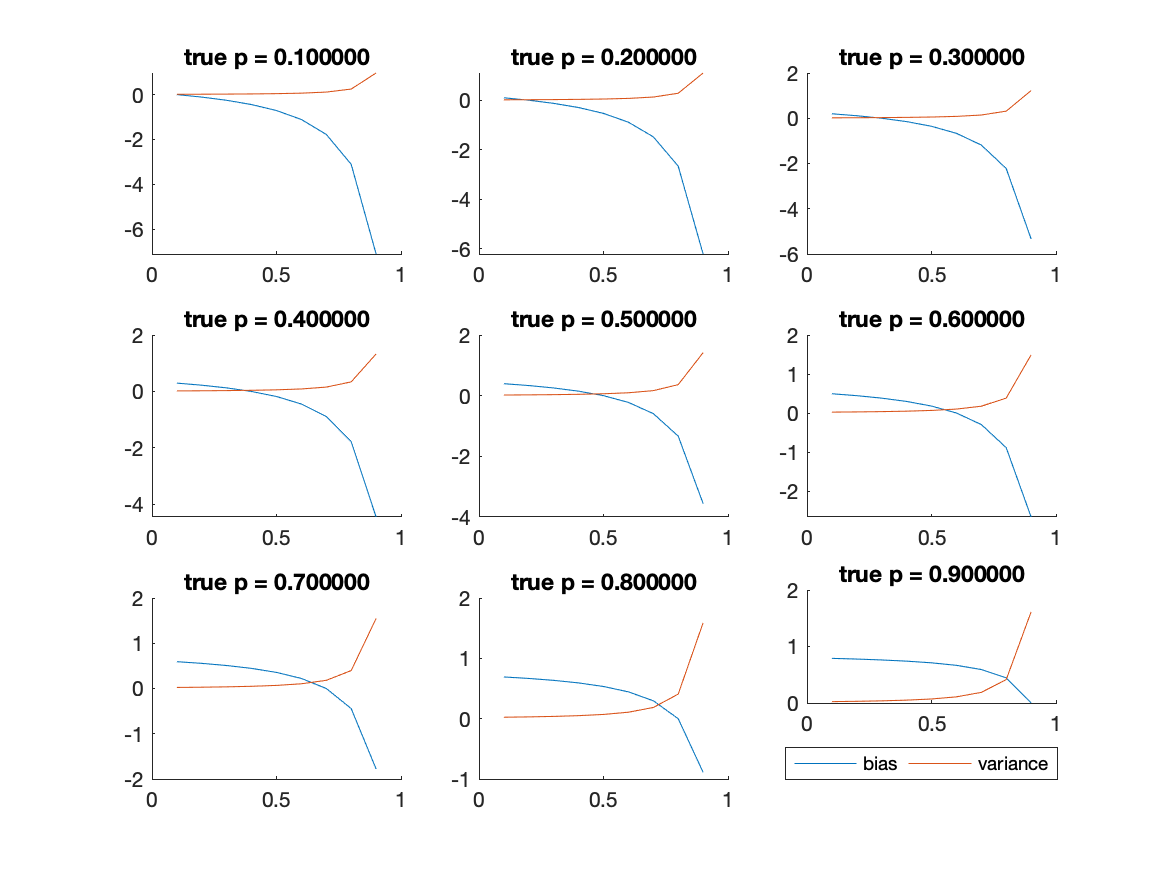
\includegraphics[width=\textwidth]{a1_2.png}

    \label{fig:my_label}
\end{figure}

\section{Multiple $x$ and multiple $y$}
\subsection{Single match within $i$} 
We observe $\{y_{i\ell}\}_{\ell=1}^{L_i}$ and $\{x_{ij}\}_{j=1}^{J_i}$ that share the same identifiers $w_i$.  As before, we assume $P(y_{i\ell}$ and $x_{ij}$ are a match $\vert w_i, L_i, J_i$) = $\frac{1}{L_i J_i}$.  Interestingly, we need only condition on the joint value $L_iJ_i$.  

\begin{align*}
    E\left[\sumL \sumJ m(y_{i\ell}, x_{ij}; \theta) \Bigg\vert w_i, L_i, J_i \right] &= \sumL \sumJ E\left[m(y_{i\ell}, x_{ij}; \theta) \vert  \text{ true match},w_i, L_i, J_i\right] P\left( \text{true match} \vert w_i,L_i, J_i\right) \\
    &+ \sumL \sumJ E\left[m(y_{i\ell}, x_{ij}; \theta) \vert  \text{ false match},w_i, L_i, J_i\right] P\left( \text{false match} \vert w_i,L_i, J_i\right) \\
    &= \frac{1}{L_i J_i} \sumL \sumJ E\left[m(y_{i\ell}, x_{ij}; \theta) \vert  \text{ true match}, w_i,L_i, J_i\right] \\
    &+ \frac{L_iJ_i - 1}{L_iJ_i}\sumL \sumJ E\left[m(y_{i\ell}, x_{ij}; \theta) \vert  \text{ false match}, w_i,L_i, J_i\right]
\end{align*}
Rearranging and using random sampling, 
\begin{align*} E\left[m(y_{i\ell}, x_{ij}; \theta) \vert  \text{ true match}, w_i, L_i, J_i\right] &=  E\left[\sumL \sumJ m(y_{i\ell}, x_{ij}; \theta) \Bigg\vert  w_i,L_i, J_i \right] \\ &- (L_iJ_i - 1)E\left[m(y_{i\ell}, x_{ij}; \theta) \vert  \text{ false match}, w_i,L_i, J_i\right]
\end{align*}
When $y_{i\ell}$ and $x_{ij}$ are not associated with the same individual (but share a same $w_i$) they are independent conditional on $w_i, L_i, J_i$.  Consider linear IV. Then:
\begin{align*} E[z_{ij}(y_{i\ell} - x_{ij}'\beta) | w_i, L_i, J_i, \text{false match} ]  &= E[z_{ij} | w_i, L_i, J_i]E[y_{i\ell} | w_i, L_i, J_i] \\
&- E[z_{ij}x_{ij}'\beta | w_i, L_i, J_i]
\end{align*}
which can be estimated using $g_z(w)g_y(w) - g_{zx}(w)\beta$.  Dimension of conditional expectations to estimate is larger.

Finally, using the law of iterated expectations
\begin{equation}
E\left[m(y_{i\ell}, x_{ij}; \theta) | \text{true match} \right] = E\left[\sumL \sumJ m(y_{i\ell}, x_{ij}; \theta)\right] - E[(L_i J_i - 1)g(w_i, L_i, J_i, \theta)]
\end{equation}
If $L_i = 1$ or $J_i = 1$ this collapses to exactly what we had before.  

Interesting to think about tradeoff in including $i$ with large $L_iJ_i$ vs. excluding.  i.e. what is signal-noise (bias-variance) tradeoff involved in this decision.  Should there be a threshold, similar to that for calling $w_i$ the same?  When is this method good? 

\subsection{Multiple matches within same $i$}

If we believe that there are $\min\{J_i, L_i\}$ pairs among the observations with matching identifier $w_i$, then $P(y_{i\ell}, x_{ij}  \text{ a match} | L_i, J_i, w_i) = \frac{\min\{J_i, L_i\}}{L_iJ_i}$, and we get
\begin{align*}  
E\left[\sumL \sumJ m(y_{i\ell}, x_{ij}; \theta) \Bigg\vert w_i, L_i, J_i \right] &= \frac{\min\{J_i, L_i\}}{L_iJ_i} \sumL \sumJ E\left[m(y_{i\ell}, x_{ij}; \theta) \vert  \text{ true match}, w_i,L_i, J_i\right] \\
    &+ \frac{L_iJ_i - \min\{L_i, J_i\}}{L_iJ_i}\sumL \sumJ E\left[m(y_{i\ell}, x_{ij}; \theta) \vert  \text{ false match}, w_i,L_i, J_i\right]
\end{align*}
which implies the final moment condition,
\begin{equation}
E\left[m(y_{i\ell}, x_{ij}; \theta) | \text{true match} \right] = E\left[\min\{J_i, L_i\} \sumL \sumJ m(y_{i\ell}, x_{ij}; \theta)\right] - E[(L_i J_i - \min\{J_i, L_i\})g(w_i, L_i, J_i)]
\end{equation}

\section*{How precise does $\hat{g}$ need to be? }
I am concerned about how you might actually estimate $g$ in applications. 

\newpage

$$\hat{\theta} = \arg\min_{\theta\in\Theta} \left\{ \min_{\mathcal{Z}}   \sum_{i=1}^n q(z_i; \theta) \right\} $$  
\end{document}
